\documentclass{article}%
\usepackage[T1]{fontenc}%
\usepackage[utf8]{inputenc}%
\usepackage{lmodern}%
\usepackage{textcomp}%
\usepackage{lastpage}%
\usepackage[head=40pt,margin=0.5in,bottom=0.6in]{geometry}%
\usepackage{graphicx}%
%
\title{\textbf{Grupo de Lima rechazó intervención militar en Venezuela}}%
\author{EFE}%
\date{15/09/2018}%
%
\begin{document}%
\normalsize%
\maketitle%
\textbf{URL: }%
http://www.el{-}nacional.com/noticias/latinoamerica/grupo{-}lima{-}rechazo{-}intervencion{-}militar{-}venezuela\_251926\newline%
%
\textbf{Periodico: }%
EN, %
ID: %
251926, %
Seccion: %
Latinoamérica\newline%
%
\textbf{Palabras Claves: }%
Nicolás Maduro, Argentina, Costa Rica, Guatemala, Chile, Brasil, Paraguay, Colombia, OEA, Perú, México, Panamá\newline%
%
\textbf{Derecho: }%
CONTEXTO%
, Otros Derechos: %
NO\_TIENE%
, Sub Derechos: %
NO\_TIENE%
\newline%
%
\textbf{EP: }%
NO\newline%
\newline%
%
\textbf{\textit{El organismo que une a 12 países instó a que las medidas tomadas deben ser pacíficas}}%
\newline%
\newline%
%
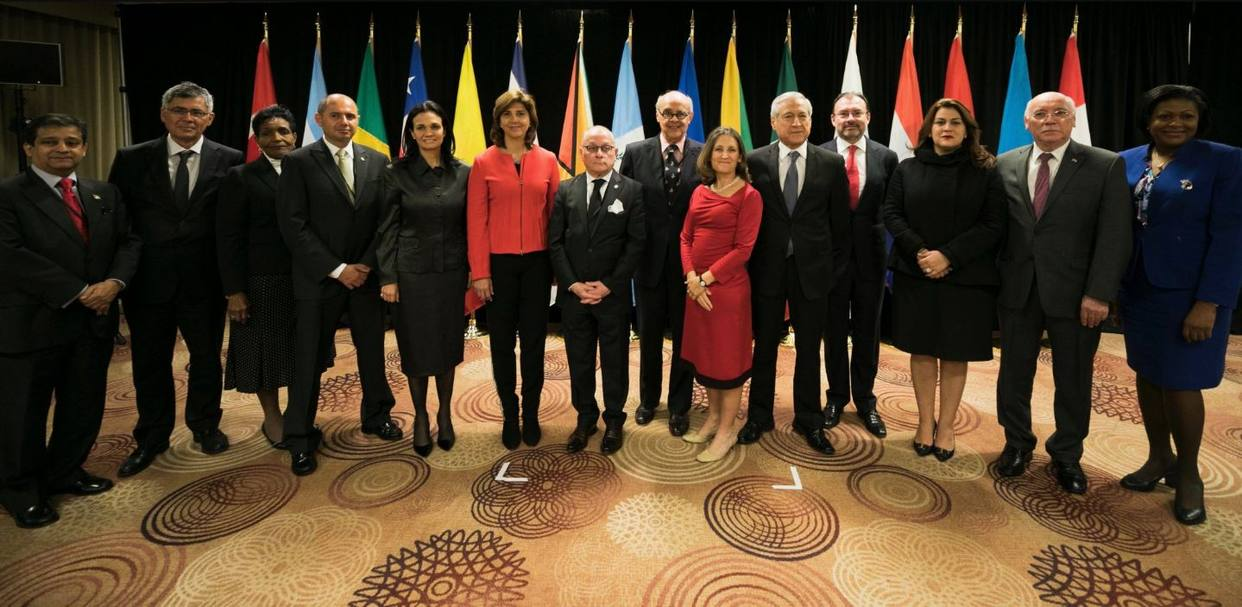
\includegraphics[width=300px]{11.jpg}%
\newline%
%
El Grupo de Lima, integrado por una docena de países latinoamericanos que considera roto el orden democrático en Venezuela, rechazó este sábado~una eventual intervención militar en esa nación, algo que no descartó este viernes el secretario general de la Organización de Estados Americanos, Luis Almagro.%
\newline%
%
Los doce países del Grupo de Lima expresaron en un comunicado conjunto "su preocupación y rechazo ante cualquier curso de acción o declaración que implique una intervención militar o el ejercicio de la violencia, la amenaza o el uso de la fuerza en Venezuela".%
\newline%
%
En ese sentido, abogaron por "una salida pacífica y negociada" para restaurar la democracia en Venezuela y a superar la "grave crisis política, económica, social y humanitaria que atraviesa ese país", por lo que reiteraron que continuarán promoviendo iniciativas para este fin en el marco del derecho internacional.%
\newline%
%
Instaron una vez más al gobierno del presidente Nicolás Maduro a "poner fin a las violaciones a los derechos humanos, a liberar a los presos políticos, respetar la autonomía de los poderes del Estado y asumir su responsabilidad por la grave crisis que hoy vive Venezuela".%
\newline%
%
En una visita este viernes a la ciudad de Cúcuta, en la frontera con Venezuela, para comprobar el masivo flujo de venezolanos que emigra a diario por la escasez de alimentos y medicinas, Almagro aseguró "que las acciones diplomáticas están en primer lugar" pero no se pueden descartar otras como la intervención militar, dada la gravedad de la situación.%
\newline%
%
En respuesta a esas palabras, el gobierno venezolano anunció que denunciará a Almagro ante Naciones Unidas por supuestamente promover una intervención militar "de forma vulgar y grotesca", según su vicepresidenta, Delcy Rodríguez.%
\newline%
%
Rodríguez consideró que la estabilidad de América Latina está "seriamente amenazada por la demencial actuación de quien usurpa de forma desviada y abusiva la secretaría general de la OEA", y~advirtió que el uruguayo "pretende revivir los peores expedientes de intervención militar imperialistas" en el continente americano.%
\newline%
%
\end{document}